%% Creator: Inkscape inkscape 0.48.4, www.inkscape.org
%% PDF/EPS/PS + LaTeX output extension by Johan Engelen, 2010
%% Accompanies image file 'areapoints.pdf' (pdf, eps, ps)
%%
%% To include the image in your LaTeX document, write
%%   \input{<filename>.pdf_tex}
%%  instead of
%%   \includegraphics{<filename>.pdf}
%% To scale the image, write
%%   \def\svgwidth{<desired width>}
%%   \input{<filename>.pdf_tex}
%%  instead of
%%   \includegraphics[width=<desired width>]{<filename>.pdf}
%%
%% Images with a different path to the parent latex file can
%% be accessed with the `import' package (which may need to be
%% installed) using
%%   \usepackage{import}
%% in the preamble, and then including the image with
%%   \import{<path to file>}{<filename>.pdf_tex}
%% Alternatively, one can specify
%%   \graphicspath{{<path to file>/}}
%% 
%% For more information, please see info/svg-inkscape on CTAN:
%%   http://tug.ctan.org/tex-archive/info/svg-inkscape
%%
\begingroup%
  \makeatletter%
  \providecommand\color[2][]{%
    \errmessage{(Inkscape) Color is used for the text in Inkscape, but the package 'color.sty' is not loaded}%
    \renewcommand\color[2][]{}%
  }%
  \providecommand\transparent[1]{%
    \errmessage{(Inkscape) Transparency is used (non-zero) for the text in Inkscape, but the package 'transparent.sty' is not loaded}%
    \renewcommand\transparent[1]{}%
  }%
  \providecommand\rotatebox[2]{#2}%
  \ifx\svgwidth\undefined%
    \setlength{\unitlength}{819.2bp}%
    \ifx\svgscale\undefined%
      \relax%
    \else%
      \setlength{\unitlength}{\unitlength * \real{\svgscale}}%
    \fi%
  \else%
    \setlength{\unitlength}{\svgwidth}%
  \fi%
  \global\let\svgwidth\undefined%
  \global\let\svgscale\undefined%
  \makeatother%
  \begin{picture}(1,0.75)%
\tiny
    \put(0,0.05){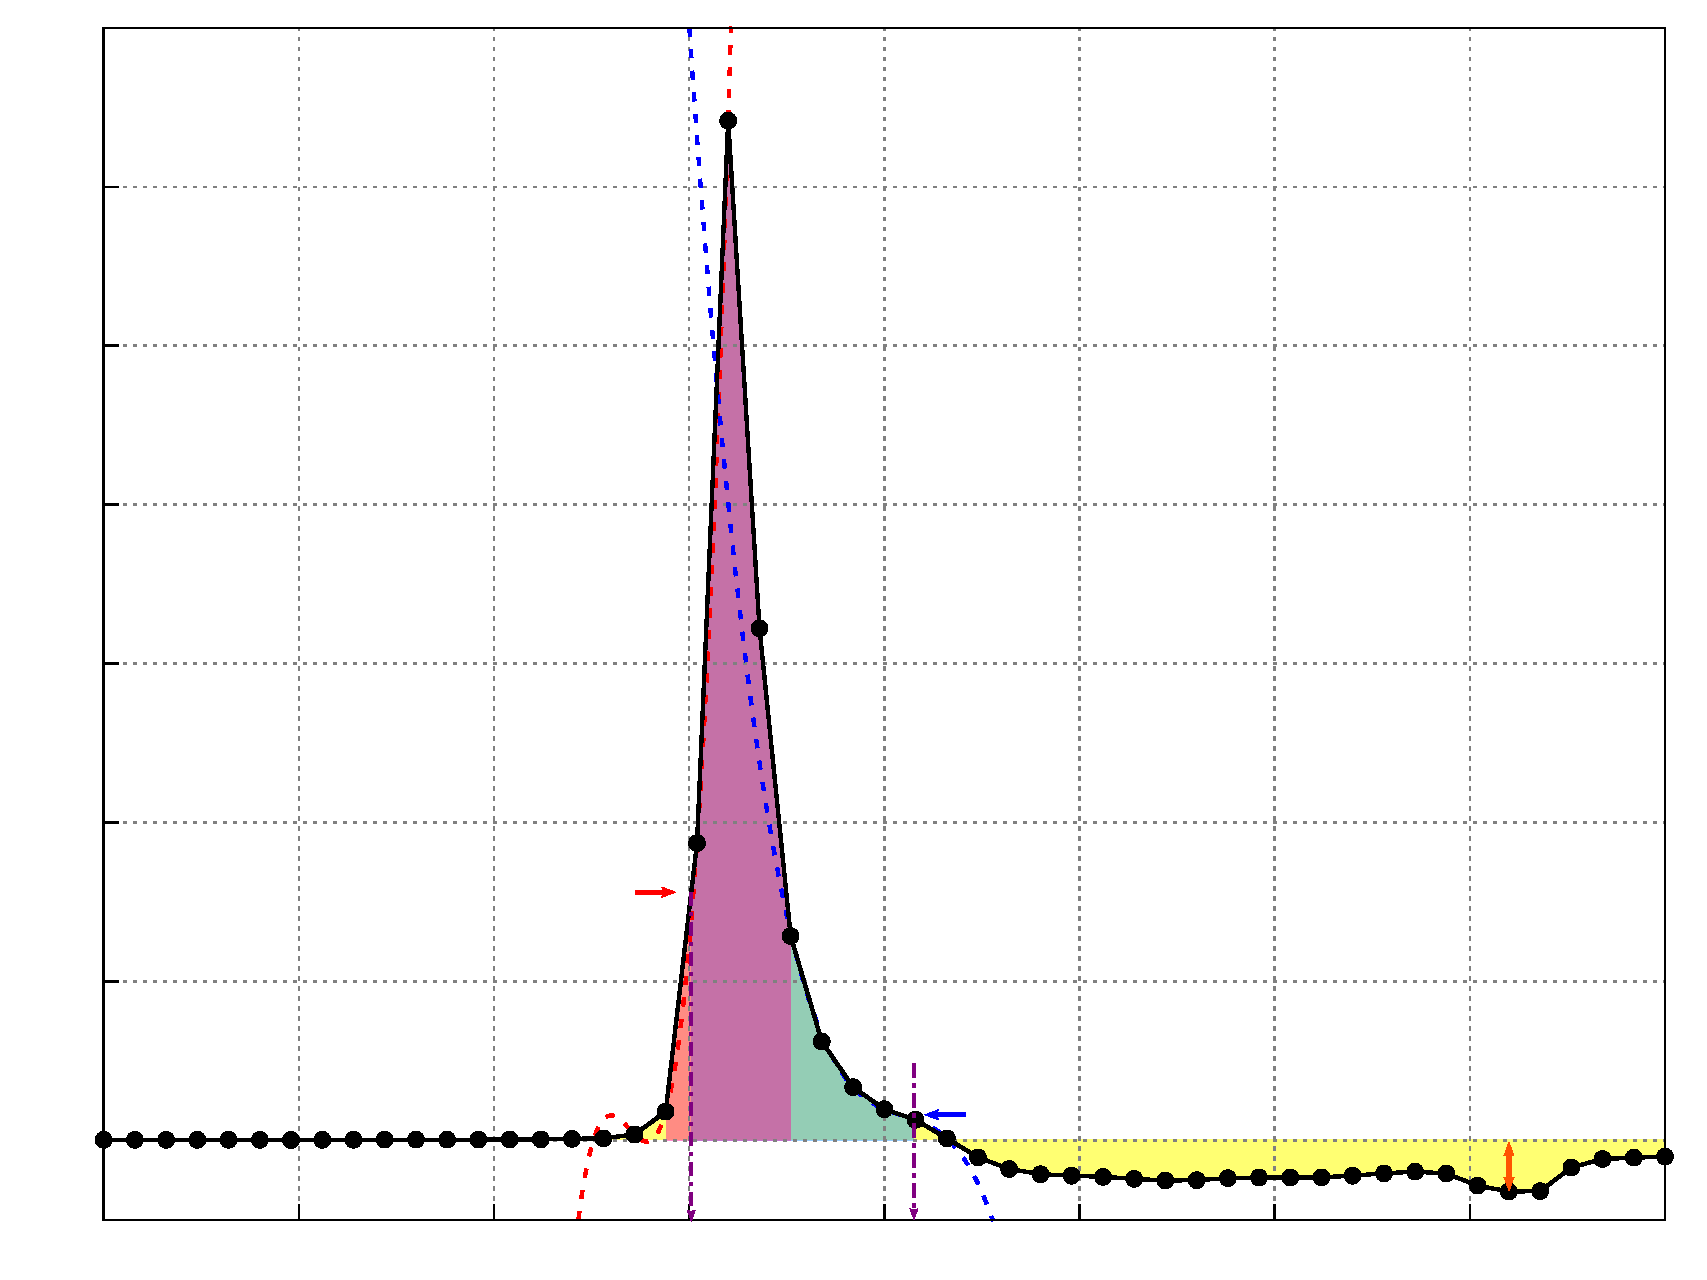
\includegraphics[width=\unitlength]{areapoints}}%
    \put(0.05263672,0.12734375){\makebox(0,0)[rb]{\smash{0}}}%
    \put(0.05263672,0.22050781){\makebox(0,0)[rb]{\smash{0.02}}}%
    \put(0.05263672,0.31357422){\makebox(0,0)[rb]{\smash{0.04}}}%
    \put(0.05263672,0.40673828){\makebox(0,0)[rb]{\smash{0.06}}}%
    \put(0.05263672,0.49990234){\makebox(0,0)[rb]{\smash{0.08}}}%
    \put(0.05263672,0.59306641){\makebox(0,0)[rb]{\smash{0.1}}}%
    \put(0.05263672,0.68613281){\makebox(0,0)[rb]{\smash{0.12}}}%
    \put(0.05263672,0.77929687){\makebox(0,0)[rb]{\smash{0.14}}}%
    \put(0.06074219,0.06318359){\makebox(0,0)[b]{\smash{0}}}%
    \put(0.17509766,0.06318359){\makebox(0,0)[b]{\smash{0.05}}}%
    \put(0.28945312,0.06318359){\makebox(0,0)[b]{\smash{0.1}}}%
    \put(0.40380859,0.06318359){\makebox(0,0)[b]{\smash{0.15}}}%
    \put(0.51816406,0.06318359){\makebox(0,0)[b]{\smash{0.2}}}%
    \put(0.63251953,0.06318359){\makebox(0,0)[b]{\smash{0.25}}}%
    \put(0.746875,0.06318359){\makebox(0,0)[b]{\smash{0.3}}}%
    \put(0.86123047,0.06318359){\makebox(0,0)[b]{\smash{0.35}}}%
    \put(0.97558594,0.06318359){\makebox(0,0)[b]{\smash{0.4}}}%
\tiny
    \put(0.20381636,0.26921044){\color[rgb]{1,0,0}\makebox(0,0)[lb]{\smash{25\% peak}}}%
    \put(0.56684619,0.13880459){\color[rgb]{0,0,1}\makebox(0,0)[lb]{\smash{5\% peak}}}%
    \put(0.87000793,0.13574677){\color[rgb]{1,0.3254902,0}\makebox(0,0)[lb]{\smash{Valley}}}%
    \put(0.53644729,0.08962654){\color[rgb]{0,0,0}\makebox(0,0)[lb]{\smash{End}}}%
    \put(0.40794882,0.08962654){\color[rgb]{0,0,0}\makebox(0,0)[lb]{\smash{Start}}}%
\scriptsize
    \put(0.48622882,0.19737821){\color[rgb]{0.11372549,0.34117647,1}\makebox(0,0)[lb]{\bfseries \smash{Energy}}}%
    \put(0.73531782,0.13898306){\color[rgb]{0.3137,0.3137,0}\makebox(0,0)[lb]{\bfseries \smash{Area}}}%
    \put(0.23328196,0.15108938){\color[rgb]{1,0,0.22352941}\makebox(0,0)[lb]{\bfseries \smash{Charge}}}%
    \put(0.5,0.01){\makebox(0,0)[b]{\smash{Time ($\mu$s)}}}%
    \put(-0.05,0.45){\rotatebox{-270}{\makebox(0,0)[b]{\smash{Voltage (V)}}}}%

  \end{picture}%
\endgroup%
